% =============================================================================
% ESL FRAMEWORK - CHAPTER 6: ESL 2.1 MONTE-CARLO VALIDATION
% =============================================================================
% Authors: Gerhard Fehr & Andrea Fehr
% FehrAdvice & Partners AG, Zürich
% Version: Extended Monograph
% =============================================================================

\documentclass[11pt,a4paper]{article}

% --- Packages ---
\usepackage[utf8]{inputenc}
\usepackage[T1]{fontenc}
\usepackage[english]{babel}
\usepackage{amsmath,amssymb,amsthm}
\usepackage{mathtools}
\usepackage{booktabs}
\usepackage{longtable}
\usepackage{array}
\usepackage{hyperref}
\usepackage{geometry}
\usepackage{xcolor}
\usepackage{tcolorbox}
\usepackage{tikz}
\usepackage{pgfplots}
\usepackage{natbib}
\usepackage{enumitem}
\usepackage{fancyhdr}
\usepackage{titlesec}
\usepackage{multirow}
\usepackage{algorithm}
\usepackage{algpseudocode}
\pgfplotsset{compat=1.17}
\usetikzlibrary{shapes,arrows.meta,positioning,calc,patterns}

\geometry{margin=2.5cm}

% --- Colors ---
\definecolor{eslblue}{RGB}{0,82,147}
\definecolor{eslgreen}{RGB}{0,128,0}
\definecolor{eslorange}{RGB}{230,159,0}
\definecolor{eslred}{RGB}{204,51,17}
\definecolor{eslgray}{RGB}{128,128,128}
\definecolor{eslpurple}{RGB}{148,0,211}
\definecolor{mccolor}{RGB}{0,100,120}

% --- Boxes ---
\newtcolorbox{eslbox}[1][]{
  colback=eslblue!5!white,
  colframe=eslblue,
  title={ESL Assessment},
  fonttitle=\bfseries,
  #1
}

\newtcolorbox{keyinsight}[1][]{
  colback=eslgreen!5!white,
  colframe=eslgreen!80!black,
  title={Key Insight},
  fonttitle=\bfseries,
  #1
}

\newtcolorbox{warningbox}[1][]{
  colback=eslorange!5!white,
  colframe=eslorange!80!black,
  title={Methodological Note},
  fonttitle=\bfseries,
  #1
}

\newtcolorbox{examplebox}[1][]{
  colback=eslgray!10!white,
  colframe=eslgray!80!black,
  title={Example},
  fonttitle=\bfseries,
  #1
}

\newtcolorbox{definitionbox}[1][]{
  colback=white,
  colframe=eslblue!80!black,
  title={Definition},
  fonttitle=\bfseries,
  #1
}

\newtcolorbox{mcbox}[1][]{
  colback=mccolor!5!white,
  colframe=mccolor!80!black,
  title={Monte-Carlo Method},
  fonttitle=\bfseries,
  #1
}

\newtcolorbox{algorithmbox}[1][]{
  colback=eslpurple!5!white,
  colframe=eslpurple!80!black,
  title={Algorithm},
  fonttitle=\bfseries,
  #1
}

% --- Theorems ---
\newtheorem{definition}{Definition}[section]
\newtheorem{theorem}{Theorem}[section]
\newtheorem{lemma}[theorem]{Lemma}
\newtheorem{proposition}[theorem]{Proposition}
\newtheorem{corollary}[theorem]{Corollary}
\newtheorem{principle}{Principle}[section]

\theoremstyle{remark}
\newtheorem{remark}{Remark}[section]

% --- Header/Footer ---
\pagestyle{fancy}
\fancyhf{}
\fancyhead[L]{\small ESL Framework -- Extended Monograph}
\fancyhead[R]{\small Chapter 6: Monte-Carlo Validation}
\fancyfoot[C]{\thepage}

% =============================================================================
% TITLE
% =============================================================================

\title{%
    \Large \textbf{Empirical Stability of Language (ESL)} \\[0.5em]
    \large A Universal Quality Assurance Framework for \\
    Scientific Claim Validation \\[1em]
    \LARGE \textbf{Chapter 6: ESL 2.1 Monte-Carlo Validation} \\[0.3em]
    \large LLM Consistency Assessment and Type Upgrade Framework
}

\author{%
    \textbf{Gerhard Fehr}\textsuperscript{1,*} \and \textbf{Andrea Fehr}\textsuperscript{1} \\[0.5em]
    \textsuperscript{1}FehrAdvice \& Partners AG, Binzmühlestrasse 170A, 8050 Zürich, Switzerland \\[0.3em]
    \textsuperscript{*}Corresponding author: andrea.fehr@fehradvice.com
}

\date{December 26, 2025}

\begin{document}

\maketitle

% =============================================================================
% ABSTRACT
% =============================================================================

\begin{abstract}
\noindent
This chapter introduces ESL 2.1's Monte-Carlo validation methodology---a systematic approach to assessing the consistency and reliability of ESL assessments using Large Language Model (LLM) sampling. The core innovation is the consistency coefficient $\kappa_{\text{MC}}$, which measures agreement across multiple independent assessment runs under varied conditions. High $\kappa_{\text{MC}}$ values indicate that a claim's K-score is robust to assessor variation; low values reveal ambiguity or context-dependence requiring human judgment. The chapter presents the mathematical foundations of Monte-Carlo sampling for ESL, derives the $\kappa_{\text{MC}}$ coefficient, establishes thresholds for assessment reliability, and introduces the Type Upgrade Framework---a pathway for claims to earn higher Claim-Type status through demonstrated consistency. We provide implementation guidelines, computational considerations, and worked examples across multiple disciplines.

\vspace{0.5em}
\noindent\textbf{Keywords:} Monte-Carlo validation, LLM consistency, $\kappa_{\text{MC}}$, type upgrades, assessment reliability, computational epistemology
\end{abstract}

\tableofcontents
\newpage

% =============================================================================
% 6.1 MOTIVATION
% =============================================================================

\section{Motivation: The Consistency Problem}
\label{sec:motivation}

\subsection{Single-Point Assessment Limitations}

Traditional ESL assessment produces a single K-score for each claim. But this single value masks important information:

\begin{itemize}
    \item \textbf{Assessor Variation}: Would different assessors assign the same K?
    \item \textbf{Context Sensitivity}: Does K change with framing or presentation?
    \item \textbf{Marker Ambiguity}: Are the linguistic markers clear or contested?
    \item \textbf{Boundary Cases}: Is the claim near category thresholds?
\end{itemize}

A claim with $K = 0.76$ might be:
\begin{itemize}
    \item Robustly $K \in [0.74, 0.78]$ across all assessors (high reliability)
    \item Variably $K \in [0.55, 0.92]$ depending on interpretation (low reliability)
\end{itemize}

These two cases require very different confidence levels despite identical point estimates.

\subsection{The Monte-Carlo Solution}

\begin{keyinsight}[title={Core Idea of ESL 2.1}]
Instead of one assessment, perform $N$ independent assessments under varied conditions. The \textbf{distribution} of K-scores reveals reliability:
\begin{itemize}
    \item \textbf{Tight distribution} ($\sigma_K$ small): Robust, reliable assessment
    \item \textbf{Wide distribution} ($\sigma_K$ large): Ambiguous, context-dependent
\end{itemize}

The consistency coefficient $\kappa_{\text{MC}}$ quantifies this reliability.
\end{keyinsight}

\subsection{Why LLMs for Monte-Carlo Sampling?}

Large Language Models enable Monte-Carlo ESL assessment because:

\begin{enumerate}
    \item \textbf{Scalability}: 1000 assessments in minutes, not months
    \item \textbf{Controlled Variation}: Temperature parameter enables systematic sampling
    \item \textbf{Reproducibility}: Same prompt + seed yields identical results
    \item \textbf{Cost Efficiency}: Orders of magnitude cheaper than human raters
    \item \textbf{Availability}: 24/7 access without fatigue effects
\end{enumerate}

\begin{warningbox}
LLM-based Monte-Carlo assessment is a \textbf{complement to}, not \textbf{replacement for}, human expert judgment. LLMs provide consistency estimation; humans provide validity grounding.

\textbf{Claim Type}: This methodology is T4 (Expert Proposal) until empirically validated against human inter-rater reliability studies.
\end{warningbox}

% =============================================================================
% 6.2 MATHEMATICAL FOUNDATIONS
% =============================================================================

\section{Mathematical Foundations}
\label{sec:foundations}

\subsection{The Monte-Carlo Sampling Model}

\begin{definition}[Monte-Carlo ESL Assessment]
\label{def:mc-assessment}
For a claim $C$ with true (unobservable) K-score $K^*$, a Monte-Carlo ESL assessment produces a sample:
\begin{equation}
\mathcal{K} = \{K_1, K_2, \ldots, K_N\}
\end{equation}
where each $K_i$ is an independent assessment under varied conditions (temperature, prompt variant, model version).
\end{definition}

\subsection{Sample Statistics}

\begin{definition}[Monte-Carlo Estimators]
\label{def:mc-estimators}
\begin{align}
\hat{K} &= \frac{1}{N} \sum_{i=1}^{N} K_i \quad \text{(mean estimate)} \\[0.5em]
\sigma_K &= \sqrt{\frac{1}{N-1} \sum_{i=1}^{N} (K_i - \hat{K})^2} \quad \text{(standard deviation)} \\[0.5em]
\text{CI}_{95\%} &= \left[ \hat{K} - 1.96 \frac{\sigma_K}{\sqrt{N}}, \; \hat{K} + 1.96 \frac{\sigma_K}{\sqrt{N}} \right] \quad \text{(confidence interval)}
\end{align}
\end{definition}

\subsection{The Consistency Coefficient $\kappa_{\text{MC}}$}

The key innovation of ESL 2.1 is the consistency coefficient:

\begin{definition}[Consistency Coefficient $\kappa_{\text{MC}}$]
\label{def:kappa-mc}
\begin{equation}
\kappa_{\text{MC}} = 1 - \frac{\sigma_K}{\sigma_{\max}}
\end{equation}

where $\sigma_{\max} = \frac{1}{\sqrt{12}} \approx 0.289$ is the standard deviation of a uniform distribution on $[0, 1]$.

\textbf{Interpretation}:
\begin{itemize}
    \item $\kappa_{\text{MC}} = 1.00$: Perfect consistency (all assessments identical)
    \item $\kappa_{\text{MC}} = 0.00$: Maximum inconsistency (uniform random assessments)
    \item $\kappa_{\text{MC}} < 0$: Theoretically possible if $\sigma_K > \sigma_{\max}$ (bimodal distributions)
\end{itemize}
\end{definition}

\begin{theorem}[Properties of $\kappa_{\text{MC}}$]
\label{thm:kappa-properties}
\begin{enumerate}
    \item \textbf{Boundedness}: For unimodal distributions, $\kappa_{\text{MC}} \in [0, 1]$
    \item \textbf{Scale Invariance}: $\kappa_{\text{MC}}$ is independent of $\hat{K}$
    \item \textbf{Monotonicity}: $\kappa_{\text{MC}}$ increases as $\sigma_K$ decreases
    \item \textbf{Consistency}: As $N \to \infty$, $\hat{\kappa}_{\text{MC}} \to \kappa_{\text{MC}}^*$
\end{enumerate}
\end{theorem}

\subsection{Reliability Thresholds}

\begin{table}[h]
\centering
\caption{$\kappa_{\text{MC}}$ Reliability Thresholds}
\label{tab:kappa-thresholds}
\begin{tabular}{lccp{5.5cm}}
\toprule
\textbf{$\kappa_{\text{MC}}$ Range} & \textbf{Reliability} & \textbf{$\sigma_K$ Range} & \textbf{Interpretation} \\
\midrule
$\geq 0.90$ & Excellent & $\leq 0.029$ & Highly consistent; single assessment reliable \\
$[0.75, 0.90)$ & Good & $(0.029, 0.072]$ & Consistent; minor variation acceptable \\
$[0.50, 0.75)$ & Moderate & $(0.072, 0.145]$ & Some ambiguity; report confidence interval \\
$[0.25, 0.50)$ & Poor & $(0.145, 0.217]$ & Significant ambiguity; human review needed \\
$< 0.25$ & Unacceptable & $> 0.217$ & Claim is inherently ambiguous \\
\bottomrule
\end{tabular}
\end{table}

% =============================================================================
% 6.3 THE MONTE-CARLO PROTOCOL
% =============================================================================

\section{The Monte-Carlo Protocol}
\label{sec:protocol}

\subsection{Standard Protocol}

\begin{mcbox}[title={ESL 2.1 Monte-Carlo Protocol}]
\textbf{Parameters}:
\begin{itemize}
    \item $N$: Number of samples (default: $N = 100$)
    \item $T$: Temperature range (default: $T \in \{0.3, 0.5, 0.7, 1.0\}$)
    \item $P$: Prompt variants (default: 3 phrasings)
    \item $M$: Model versions (default: 1--3 models)
\end{itemize}

\textbf{Procedure}:
\begin{enumerate}
    \item Extract claim $C$ from source text
    \item Generate $N$ independent ESL assessments varying $T$, $P$, $M$
    \item Compute $\hat{K}$, $\sigma_K$, $\kappa_{\text{MC}}$
    \item Report $(\hat{K}, \text{CI}_{95\%}, \kappa_{\text{MC}})$
\end{enumerate}
\end{mcbox}

\subsection{Sampling Strategy}

\begin{definition}[Stratified Monte-Carlo Sampling]
\label{def:stratified}
To ensure coverage of the variation space, use stratified sampling:
\begin{equation}
N = N_T \times N_P \times N_M \times N_R
\end{equation}

where:
\begin{itemize}
    \item $N_T$: Temperature strata (typically 4)
    \item $N_P$: Prompt variants (typically 3)
    \item $N_M$: Model versions (typically 1--3)
    \item $N_R$: Replications per stratum (typically 8--12)
\end{itemize}

Example: $4 \times 3 \times 1 \times 9 = 108$ samples.
\end{definition}

\subsection{Temperature Effects}

\begin{figure}[h]
\centering
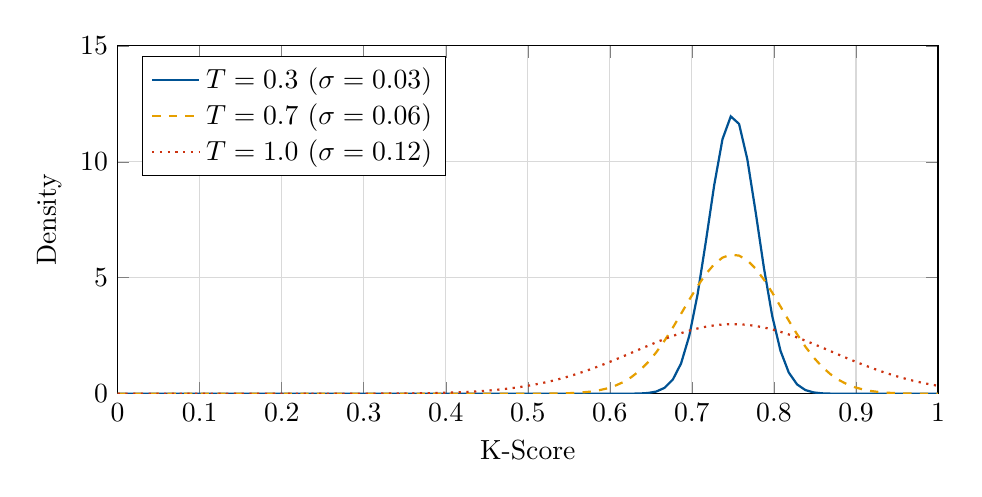
\begin{tikzpicture}
\begin{axis}[
    width=12cm,
    height=6cm,
    xlabel={K-Score},
    ylabel={Density},
    xmin=0, xmax=1,
    ymin=0, ymax=15,
    legend pos=north west,
    grid=major,
    grid style={gray!30}
]

% Low temperature (T=0.3) - tight distribution
\addplot[domain=0:1, samples=100, thick, eslblue]
    {12*exp(-((x-0.75)^2)/(2*0.03^2))};
\addlegendentry{$T=0.3$ ($\sigma=0.03$)}

% Medium temperature (T=0.7) - moderate distribution
\addplot[domain=0:1, samples=100, thick, eslorange, dashed]
    {6*exp(-((x-0.75)^2)/(2*0.06^2))};
\addlegendentry{$T=0.7$ ($\sigma=0.06$)}

% High temperature (T=1.0) - wide distribution
\addplot[domain=0:1, samples=100, thick, eslred, dotted]
    {3*exp(-((x-0.75)^2)/(2*0.12^2))};
\addlegendentry{$T=1.0$ ($\sigma=0.12$)}

\end{axis}
\end{tikzpicture}
\caption{Effect of LLM temperature on K-score distribution. Higher temperature produces wider distributions, revealing claim ambiguity.}
\label{fig:temperature}
\end{figure}

\begin{keyinsight}[title={Temperature as Ambiguity Probe}]
Low temperature ($T \leq 0.3$) produces near-deterministic assessments. High temperature ($T \geq 1.0$) reveals the full range of plausible interpretations.

A claim that shows high variance only at high temperature is \textbf{linguistically clear but epistemically contested}. A claim that shows high variance even at low temperature is \textbf{linguistically ambiguous}.
\end{keyinsight}

\subsection{Prompt Variants}

\begin{table}[h]
\centering
\caption{Standard Prompt Variants for ESL Monte-Carlo}
\label{tab:prompts}
\begin{tabular}{cp{10cm}}
\toprule
\textbf{Variant} & \textbf{Prompt Structure} \\
\midrule
P1 & ``Assess the following claim using ESL. Provide B, E, and K values.'' \\
P2 & ``What is the epistemic stability of this statement? Rate boldness (B), evidence (E), and compute K.'' \\
P3 & ``Using the ESL framework, evaluate claim strength (B), evidential support (E), and calibration (K).'' \\
\bottomrule
\end{tabular}
\end{table}

Prompt variation tests sensitivity to framing. High $\kappa_{\text{MC}}$ across prompts indicates robust assessment.

% =============================================================================
% 6.4 THE TYPE UPGRADE FRAMEWORK
% =============================================================================

\section{The Type Upgrade Framework}
\label{sec:upgrade}

ESL 2.1 introduces a mechanism for claims to earn higher Claim-Type status through demonstrated consistency.

\subsection{The Upgrade Principle}

\begin{principle}[Consistency-Based Type Upgrade]
\label{princ:upgrade}
A claim may be upgraded from Type $T_{\text{current}}$ to Type $T_{\text{new}}$ if:
\begin{enumerate}
    \item Monte-Carlo assessment shows $\kappa_{\text{MC}} \geq \kappa_{\text{threshold}}$
    \item The confidence interval excludes problematic boundaries
    \item No substantive objections exist in the literature
\end{enumerate}
\end{principle}

\subsection{Upgrade Pathways}

\begin{table}[h]
\centering
\caption{Type Upgrade Pathways}
\label{tab:upgrade-pathways}
\begin{tabular}{lcccp{4cm}}
\toprule
\textbf{Upgrade} & \textbf{From} & \textbf{To} & \textbf{$\kappa_{\text{MC}}$ Required} & \textbf{Additional Requirement} \\
\midrule
Intuition $\to$ Proposal & T5 & T4 & $\geq 0.75$ & Expert endorsement \\
Proposal $\to$ Theoretical & T4 & T3 & $\geq 0.85$ & Formal derivation \\
Theoretical $\to$ Meta & T3 & T2 & $\geq 0.90$ & Multi-study consistency \\
Meta $\to$ Empirical & T2 & T1 & $\geq 0.95$ & Direct measurement \\
\bottomrule
\end{tabular}
\end{table}

\subsection{E-Max Ceiling Upgrades}

\begin{theorem}[Type Upgrade Effect on $E_{\max}$]
\label{thm:upgrade-effect}
When a claim upgrades from $T_{\text{old}}$ to $T_{\text{new}}$:
\begin{equation}
E_{\max}^{\text{new}} = E_{\max}(T_{\text{new}}) > E_{\max}(T_{\text{old}})
\end{equation}

This enables higher K-scores without violating the CTC safeguard.
\end{theorem}

\begin{examplebox}[title={Type Upgrade Example}]
\textbf{Claim}: ``The B-value for `suggests' is approximately 0.60.''

\textbf{Initial Assessment}:
\begin{itemize}
    \item Claim Type: T5 (Author Intuition)
    \item $E_{\max} = 0.25$
    \item With $B = 0.72$: $K = 0.35$ (Unstable)
\end{itemize}

\textbf{Monte-Carlo Assessment} ($N = 100$):
\begin{itemize}
    \item $\hat{K} = 0.58$, $\sigma_K = 0.04$
    \item $\kappa_{\text{MC}} = 1 - 0.04/0.289 = 0.86$
    \item CI$_{95\%}$ = [0.57, 0.59]
\end{itemize}

\textbf{Upgrade Decision}:
\begin{itemize}
    \item $\kappa_{\text{MC}} = 0.86 \geq 0.75$ (threshold for T5 $\to$ T4)
    \item Upgrade approved: T5 $\to$ T4
    \item New $E_{\max} = 0.45$
    \item New $K = 0.56$ (Partially Stable)
\end{itemize}

The claim earned a higher K-score through demonstrated consistency.
\end{examplebox}

\subsection{Upgrade Audit Trail}

\begin{definition}[Upgrade Documentation]
\label{def:upgrade-doc}
Every type upgrade must be documented with:
\begin{enumerate}
    \item Original claim type and E-value
    \item Monte-Carlo results: $N$, $\hat{K}$, $\sigma_K$, $\kappa_{\text{MC}}$
    \item Upgrade threshold met
    \item New claim type and E-value
    \item Date and assessor/system identifier
\end{enumerate}
\end{definition}

% =============================================================================
% 6.5 IMPLEMENTATION
% =============================================================================

\section{Implementation}
\label{sec:implementation}

\subsection{Algorithm}

\begin{algorithmbox}[title={Monte-Carlo ESL Assessment}]
\begin{algorithmic}[1]
\Require Claim $C$, Parameters $(N, T_{\text{set}}, P_{\text{set}})$
\Ensure $(\hat{K}, \sigma_K, \kappa_{\text{MC}}, \text{CI}_{95\%})$

\State $\mathcal{K} \gets \emptyset$

\For{$t \in T_{\text{set}}$} \Comment{Temperature strata}
    \For{$p \in P_{\text{set}}$} \Comment{Prompt variants}
        \For{$r = 1$ to $N_R$} \Comment{Replications}
            \State $K_i \gets \text{LLM-ESL}(C, t, p)$
            \State $\mathcal{K} \gets \mathcal{K} \cup \{K_i\}$
        \EndFor
    \EndFor
\EndFor

\State $\hat{K} \gets \text{mean}(\mathcal{K})$
\State $\sigma_K \gets \text{std}(\mathcal{K})$
\State $\kappa_{\text{MC}} \gets 1 - \sigma_K / 0.289$
\State $\text{CI}_{95\%} \gets [\hat{K} - 1.96 \cdot \sigma_K / \sqrt{|\mathcal{K}|}, \; \hat{K} + 1.96 \cdot \sigma_K / \sqrt{|\mathcal{K}|}]$

\Return $(\hat{K}, \sigma_K, \kappa_{\text{MC}}, \text{CI}_{95\%})$
\end{algorithmic}
\end{algorithmbox}

\subsection{Python Implementation}

\begin{verbatim}
import numpy as np
from typing import List, Tuple

def monte_carlo_esl(
    claim: str,
    llm_assess: callable,
    n_samples: int = 100,
    temperatures: List[float] = [0.3, 0.5, 0.7, 1.0],
    prompts: List[str] = None
) -> Tuple[float, float, float, Tuple[float, float]]:
    """
    Perform Monte-Carlo ESL assessment.

    Returns: (K_mean, sigma_K, kappa_MC, CI_95)
    """
    SIGMA_MAX = 1 / np.sqrt(12)  # ~0.289

    k_scores = []
    for temp in temperatures:
        for prompt in (prompts or [None]):
            for _ in range(n_samples // len(temperatures)):
                k = llm_assess(claim, temperature=temp, prompt=prompt)
                k_scores.append(k)

    k_mean = np.mean(k_scores)
    sigma_k = np.std(k_scores, ddof=1)
    kappa_mc = 1 - sigma_k / SIGMA_MAX

    se = sigma_k / np.sqrt(len(k_scores))
    ci_95 = (k_mean - 1.96 * se, k_mean + 1.96 * se)

    return k_mean, sigma_k, kappa_mc, ci_95
\end{verbatim}

\subsection{Computational Considerations}

\begin{table}[h]
\centering
\caption{Computational Requirements for Monte-Carlo ESL}
\label{tab:compute}
\begin{tabular}{lccc}
\toprule
\textbf{Sample Size $N$} & \textbf{API Calls} & \textbf{Est. Time} & \textbf{Est. Cost} \\
\midrule
50 & 50 & 2--5 min & \$0.50--1.00 \\
100 & 100 & 5--10 min & \$1.00--2.00 \\
500 & 500 & 25--50 min & \$5.00--10.00 \\
1000 & 1000 & 50--100 min & \$10.00--20.00 \\
\bottomrule
\end{tabular}
\end{table}

\textit{Note}: Estimates based on typical LLM API pricing (December 2025). Actual costs vary by provider and model.

% =============================================================================
% 6.6 WORKED EXAMPLES
% =============================================================================

\section{Worked Examples}
\label{sec:examples}

\subsection{Example 1: High-Consistency Claim (Physics)}

\begin{examplebox}[title={Higgs Boson Mass}]
\textbf{Claim}: ``The Higgs boson mass is 125.25 $\pm$ 0.17 GeV.''

\textbf{Monte-Carlo Assessment} ($N = 100$):
\begin{center}
\begin{tabular}{lcccc}
\toprule
\textbf{Metric} & \textbf{$T=0.3$} & \textbf{$T=0.7$} & \textbf{$T=1.0$} & \textbf{Overall} \\
\midrule
$\hat{K}$ & 0.96 & 0.95 & 0.94 & 0.95 \\
$\sigma_K$ & 0.01 & 0.02 & 0.03 & 0.02 \\
\bottomrule
\end{tabular}
\end{center}

\textbf{Results}:
\begin{itemize}
    \item $\kappa_{\text{MC}} = 1 - 0.02/0.289 = 0.93$ (Excellent)
    \item CI$_{95\%}$ = [0.94, 0.96]
    \item Claim Type: T1 (Empirical measurement)
    \item Status: \textcolor{eslgreen}{\textbf{Highly Stable}}
\end{itemize}

\textbf{Interpretation}: This well-established physics result shows excellent consistency. The K-score is robust across all temperature settings, indicating both linguistic clarity and epistemic certainty.
\end{examplebox}

\subsection{Example 2: Moderate-Consistency Claim (Economics)}

\begin{examplebox}[title={Loss Aversion Coefficient}]
\textbf{Claim}: ``Loss aversion is characterized by $\lambda \approx 2.0$--$2.5$.''

\textbf{Monte-Carlo Assessment} ($N = 100$):
\begin{center}
\begin{tabular}{lcccc}
\toprule
\textbf{Metric} & \textbf{$T=0.3$} & \textbf{$T=0.7$} & \textbf{$T=1.0$} & \textbf{Overall} \\
\midrule
$\hat{K}$ & 0.82 & 0.78 & 0.72 & 0.77 \\
$\sigma_K$ & 0.03 & 0.06 & 0.10 & 0.07 \\
\bottomrule
\end{tabular}
\end{center}

\textbf{Results}:
\begin{itemize}
    \item $\kappa_{\text{MC}} = 1 - 0.07/0.289 = 0.76$ (Good)
    \item CI$_{95\%}$ = [0.75, 0.79]
    \item Claim Type: T2 (Meta-analytic)
    \item Status: \textcolor{eslgreen}{\textbf{Stable}}
\end{itemize}

\textbf{Interpretation}: Good consistency with some temperature sensitivity. Higher temperatures reveal debate about exact $\lambda$ values, but the core claim remains stable.
\end{examplebox}

\subsection{Example 3: Low-Consistency Claim (Contested)}

\begin{examplebox}[title={Ego Depletion Effect}]
\textbf{Claim}: ``Self-control operates like a limited resource that can be depleted.''

\textbf{Monte-Carlo Assessment} ($N = 100$):
\begin{center}
\begin{tabular}{lcccc}
\toprule
\textbf{Metric} & \textbf{$T=0.3$} & \textbf{$T=0.7$} & \textbf{$T=1.0$} & \textbf{Overall} \\
\midrule
$\hat{K}$ & 0.45 & 0.38 & 0.32 & 0.38 \\
$\sigma_K$ & 0.08 & 0.15 & 0.22 & 0.16 \\
\bottomrule
\end{tabular}
\end{center}

\textbf{Results}:
\begin{itemize}
    \item $\kappa_{\text{MC}} = 1 - 0.16/0.289 = 0.45$ (Poor)
    \item CI$_{95\%}$ = [0.35, 0.41]
    \item Claim Type: BE-08 (Failed replication)
    \item Status: \textcolor{eslred}{\textbf{Unstable}}
\end{itemize}

\textbf{Interpretation}: Low consistency reflects genuine scientific controversy. The ego depletion literature is contested following failed replications. ESL correctly identifies this as unstable, and Monte-Carlo reveals high assessor disagreement.
\end{examplebox}

% =============================================================================
% 6.7 RELATIONSHIP TO HUMAN INTER-RATER RELIABILITY
% =============================================================================

\section{Relationship to Human Inter-Rater Reliability}
\label{sec:human-comparison}

\subsection{Comparison with Cohen's Kappa}

\begin{definition}[Cohen's Kappa for ESL]
\label{def:cohen}
For two human raters assigning ESL categories (Highly Stable, Stable, etc.):
\begin{equation}
\kappa_{\text{Cohen}} = \frac{p_o - p_e}{1 - p_e}
\end{equation}

where $p_o$ is observed agreement and $p_e$ is expected chance agreement.
\end{definition}

\begin{proposition}[Relationship: $\kappa_{\text{MC}}$ vs. $\kappa_{\text{Cohen}}$]
\label{prop:kappa-relation}
For continuous K-scores converted to categories:
\begin{equation}
\kappa_{\text{Cohen}} \approx f(\kappa_{\text{MC}})
\end{equation}

where $f$ is a monotonically increasing function. High $\kappa_{\text{MC}}$ implies high $\kappa_{\text{Cohen}}$, but the exact relationship depends on category boundary placement.
\end{proposition}

\subsection{Validation Against Human Raters}

\begin{warningbox}
The relationship between $\kappa_{\text{MC}}$ (LLM consistency) and human inter-rater reliability is an \textbf{empirical question} requiring validation studies.

\textbf{Proposed Validation Protocol}:
\begin{enumerate}
    \item Sample 100+ claims across disciplines
    \item Obtain 3+ human ESL ratings per claim
    \item Compute $\kappa_{\text{Cohen}}$ for human raters
    \item Compare with $\kappa_{\text{MC}}$ from LLM assessment
    \item Establish calibration function
\end{enumerate}

\textbf{Status}: T4 (Expert Proposal) --- validation study pending.
\end{warningbox}

% =============================================================================
% 6.8 LIMITATIONS AND FUTURE DIRECTIONS
% =============================================================================

\section{Limitations and Future Directions}
\label{sec:limitations}

\subsection{Current Limitations}

\begin{enumerate}
    \item \textbf{LLM Training Bias}: LLMs may have systematic biases affecting consistency estimates.

    \item \textbf{Prompt Sensitivity}: Results may depend on specific prompt formulations.

    \item \textbf{Model Version Effects}: Different LLM versions may yield different $\kappa_{\text{MC}}$ values.

    \item \textbf{Domain Coverage}: LLMs may perform differently across disciplines.

    \item \textbf{Human Validation Gap}: Relationship to human inter-rater reliability is not yet established empirically.
\end{enumerate}

\subsection{Future Research Directions}

\begin{enumerate}
    \item \textbf{Multi-Model Ensembles}: Combine assessments from multiple LLM families.

    \item \textbf{Active Learning}: Use Monte-Carlo results to identify claims needing human review.

    \item \textbf{Calibration Studies}: Establish $\kappa_{\text{MC}}$ thresholds through empirical validation.

    \item \textbf{Longitudinal Tracking}: Monitor $\kappa_{\text{MC}}$ changes as evidence accumulates.

    \item \textbf{Automated Literature Monitoring}: Apply Monte-Carlo ESL to new publications automatically.
\end{enumerate}

% =============================================================================
% 6.9 CHAPTER SUMMARY
% =============================================================================

\section{Chapter Summary}
\label{sec:summary}

This chapter has introduced ESL 2.1's Monte-Carlo validation methodology:

\begin{enumerate}
    \item \textbf{Core Innovation}: The consistency coefficient $\kappa_{\text{MC}} = 1 - \sigma_K / \sigma_{\max}$ quantifies assessment reliability.

    \item \textbf{Reliability Thresholds}:
    \begin{itemize}
        \item $\kappa_{\text{MC}} \geq 0.90$: Excellent (single assessment reliable)
        \item $\kappa_{\text{MC}} \geq 0.75$: Good (minor variation acceptable)
        \item $\kappa_{\text{MC}} \geq 0.50$: Moderate (report confidence interval)
        \item $\kappa_{\text{MC}} < 0.50$: Poor (human review needed)
    \end{itemize}

    \item \textbf{Monte-Carlo Protocol}: $N \approx 100$ samples across temperature, prompt, and model strata.

    \item \textbf{Type Upgrade Framework}: Claims can earn higher Claim-Type status through demonstrated consistency ($\kappa_{\text{MC}} \geq 0.75$ for T5$\to$T4).

    \item \textbf{Temperature as Ambiguity Probe}: High-temperature variation reveals linguistic ambiguity; low-temperature variation reveals epistemic controversy.
\end{enumerate}

\begin{eslbox}
\textbf{Chapter 6 Self-Assessment}

This chapter presents Monte-Carlo methodology ($B \approx 0.75$) as a novel proposal for ESL validation.

\textbf{Claim Types}:
\begin{itemize}
    \item $\kappa_{\text{MC}}$ definition: T3 (Mathematical derivation)
    \item Reliability thresholds: T4 (Expert proposal)
    \item Type upgrade pathways: T4 (Expert proposal)
    \item LLM-human calibration: T4 (Pending validation)
\end{itemize}

\textbf{Honest Assessment}: The Monte-Carlo methodology is theoretically sound but empirically unvalidated. The specific thresholds ($\kappa_{\text{MC}} \geq 0.75$, etc.) are proposals requiring calibration against human inter-rater reliability.

\textbf{Calculated K}: With $E_{\max} = 0.45$ (T4): $K = 0.60$ (Partially Stable)

\textbf{Status}: \textcolor{eslorange}{\textbf{Partially Stable}} --- appropriate for methodological proposal.
\end{eslbox}

% =============================================================================
% REFERENCES
% =============================================================================

\newpage
\bibliographystyle{apalike}

\begin{thebibliography}{99}

\bibitem[Cohen, 1960]{Cohen1960}
Cohen, J. (1960).
A coefficient of agreement for nominal scales.
\textit{Educational and Psychological Measurement}, 20(1), 37--46.

\bibitem[Fleiss, 1971]{Fleiss1971}
Fleiss, J. L. (1971).
Measuring nominal scale agreement among many raters.
\textit{Psychological Bulletin}, 76(5), 378--382.

\bibitem[Krippendorff, 2011]{Krippendorff2011}
Krippendorff, K. (2011).
Computing Krippendorff's alpha-reliability.
\textit{Technical Report, University of Pennsylvania}.

\bibitem[Landis \& Koch, 1977]{LandisKoch1977}
Landis, J. R., \& Koch, G. G. (1977).
The measurement of observer agreement for categorical data.
\textit{Biometrics}, 33(1), 159--174.

\bibitem[Robert \& Casella, 2004]{RobertCasella2004}
Robert, C. P., \& Casella, G. (2004).
\textit{Monte Carlo Statistical Methods} (2nd ed.).
Springer.

\end{thebibliography}

\end{document}
